\chapter{\textit{GreenT} : fonctionnement général}\label{chapGreent}
\putminitoc

Comme nous l'avons montré dans le chapitre \ref{chapPb}, l'entreprise a besoin d'un nouvel outil aidant aux tests d'intégration : \textit{GreenT}. 

Nous allons donc voir le développement et la conception de cette plateforme de tests.

Au début de mon stage, le projet ayant un an, les fonctionnalités développées ci-dessous étaient déjà faites. Je suis cependant intervenu
sur la plupart d'entre elles soit pour des corrections de bogues d'une part, soit à des fin d'améliorations d'autre parts.

Avant de présenter mon travail, que vous trouverez chapitre \ref{collab}, il est nécessaire de présenter le fonctionnement général de
cette plateforme afin d'en avoir une vue d'ensemble.

\section{Le fichier Walkthrough}\label{wt}
Le fichier \textit{Walkthrough} est un fichier qui sera fourni par la personne en charge des tests, c'est un fichier au format Excel qui contient les informations
de chacune des variables à tester. Il contient ainsi un très grand nombre de colonnes, bien que seule une partie de celles-ci nous
intéressent. Certaines colonnes ont été remplies par le fournisseur du plugin, d'autres colonnes sont ajoutées dans le seul but de la
génération de tests automatiques par \textit{GreenT}. Voici les informations les plus intéressantes : 

\begin{description} 
	\item[Nom de la variable] Le nom de la variable testée : il existe un nom court et un nom long.
	\item[Informations aidant à la conversion des données] Certains équipements\footnote{Vous trouverez plus d'informations sur le fonctionnement d'une table de tests section \ref{wb}} tel que le \textit{debugger} ne fonctionne qu'avec des
	valeurs Hexadécimales. À la charge de \textit{GreenT} de convertir ces données vers des valeurs physiques exploitables par
	le testeur. Ces colonnes contiennent les informations nécessaires au calcul de conversion\footnote{Informations tel que le
		domaine de définition physique et le domaine de définition hexadécimal, avec ces deux informations il est possible d'effectuer les conversions physique vers hexadécimal}.
	\item[Nécessité d'un test automatique] Un \texttt{GreenTTest} ne sera généré que si la colonne vaut \textit{Yes}.
	\item[Statut du test] La plateforme éditera automatiquement cette colonne afin de reporter le statut du test\footnote{Un test pouvant être \textit{Green} ou \textit{Red}
		mais peut aussi comporter une erreur, tel qu'un problème d'exécution ou de génération, \ldots}.
	\item[Précondition (cf section \ref{stim})] Contient un scénario d'initialisation du \textit{workbench} : tension de départ,
	démarrage de l'ECU, \ldots
	\item[Scénario de stimulation (cf section \ref{stim})] Contient un ou plusieurs scenarii de stimulations destinés à faire générer au HiL un certain nombre de stimuli.
	\item[\texttt{ExpectedBehavior} (comportement attendu, cf section \ref{expectedBehavior})] Contient une expression évaluant les variables ayant été enregistrées durant la stimulation : \textit{GreenT} devra vérifier que cette expression est correcte à toute instant de la stimulation.
	\item[Variable à enregistrer (cf section \ref{expectedBehavior})] Contient les variables devant être enregistrées durant un
	scénario, en plus des variables présentes dans l'expected behavior. Celles-ci peuvent servir en tant que données
	contextuelles permettant de mieux cerner le résultat d'un test.
	\item[Informations du test (cf section \ref{report})] Plusieurs colonnes telles que la sévérité, le responsable du test, des commentaires, \ldots
\end{description}


\begin{figure}[H]
	% TODO CHange WT version
	\hspace{-35px}
	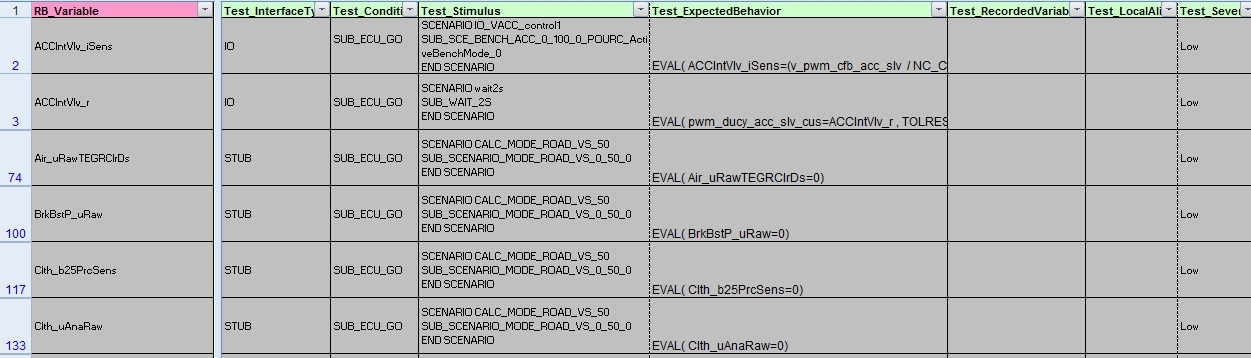
\includegraphics[width=20cm]{contents/images/walkthrough.png}
	\caption{Aperçu d'un fichier Walkthrough}
\end{figure}

\section{Fonctionnement Global}
Le développement de \textit{GreenT} inclut un certain nombre de fonctionnalités attendues par le client et indispensable à son fonctionnement. D'autres fonctionnalités pourront apparaître plus tard en fonction des besoins.

Les principaux modules sont les suivants, avec leurs interactions schématisées figure \ref{fig:generalDiag} : 
dans des objets ovales sont représentés des fichiers, les carrés représentent des modules de la plateforme et les flèches en pointillés un transfert réseau, les couleurs représentent les différents modules de la plateforme.

\begin{figure}[H]
	\hspace{-25px}
	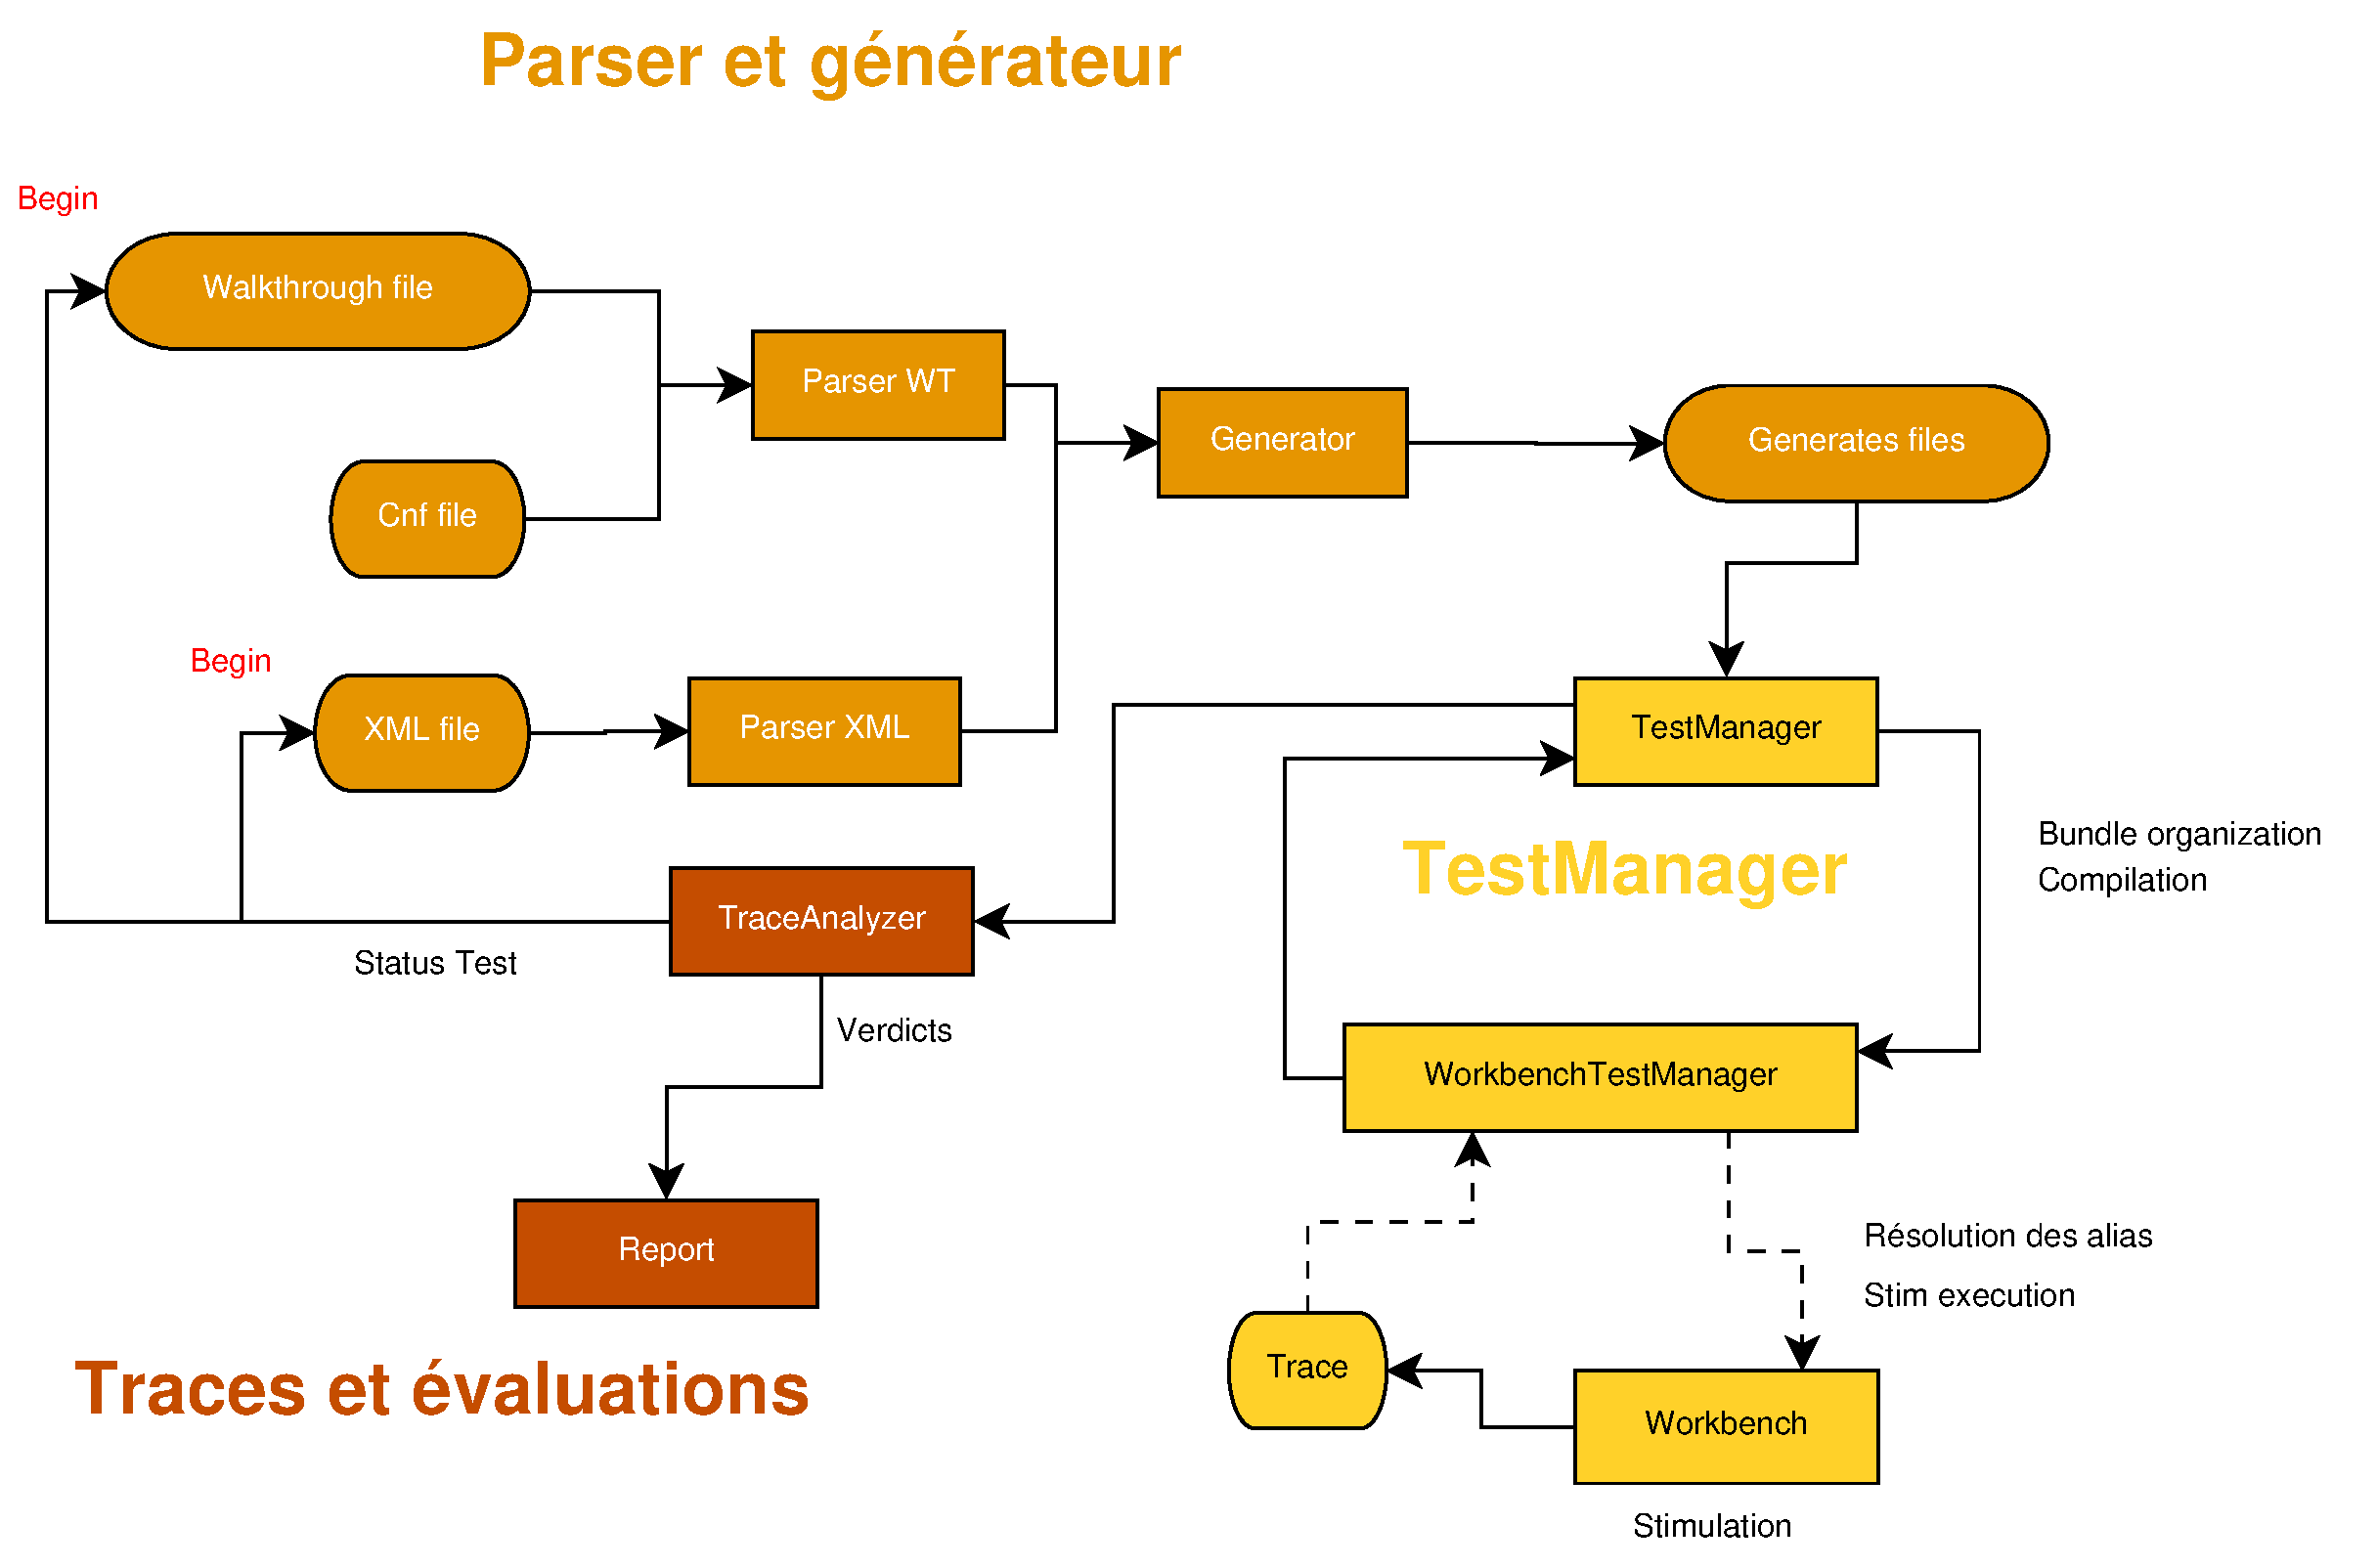
\includegraphics[width=20cm]{contents/images/generalDiag.eps}
	\caption{Fonctionnement général de la plateforme \textit{GreenT}}
	\label{fig:generalDiag}
\end{figure}	

Dans la figure \ref{fig:generalDiag}, vous pouvez voir des flèches en pointillés représentant des échanges réseau. En effet
l'exécution des stimulations et l'enregistrement des traces se fait par un contrôle distant des bancs de tests\footnote{La
	schématisation du fonctionnement d'un banc est disponible section \ref{wb} figure \ref{fig:wb}}.

Les principales fonctionnalités demandées par le client sont disponibles sur le client, la majorité peuvent s'effectuer en local : 
\begin{itemize}
	\item Le parsing et la génération (section \ref{generation})
	\item L'organisation en Bundle afin d'optimiser le temps d'exécution des tests (section \ref{testManager})
	\item La production de rapports détaillés (section \ref{expectedBehavior})
\end{itemize}~\newline
Alors que d'autres fonctionnalités vont nécessiter la présence de serveurs et de connexion réseau permettant d'effectuer ces actions
: 
\begin{itemize}
	\item Les stimulations (section \ref{stim})
	\item Les enregistrement des traces (section \ref{stim})
\end{itemize}
\vspace{-10px}
\section{Les fonctionnalités du Client}
Afin de répondre au mieux aux attentes du client, il a été choisi d'utiliser le langage Java pour développer notre client, ceci en raison de
divers avantages comme le côté multi-plateforme, son typage fort et sa forte communauté qui permet ainsi une maintenance facilitée. 

\subsection{\textit{Parsing} et Génération}\label{generation}
Le but premier de la plateforme est d'effectuer des tests automatiques, il est ainsi indispensable d'avoir un système d'automatisation, au travers d'une génération.

Pour cela, nous avons un parser : il analyse un certain type de fichier\footnote{Nous ne commencerons qu'avec le Walkthrough pour débuter, mais dans le futur nous pourrions avoir des fichiers XML, des bases de données, \ldots} et en retire pour chaque test, le scénario de pré condition, les différents scénarios de stimulations, leur \textit{Expected Behavior}, les données qui devront être enregistrées ainsi que différentes informations sur le test\footnote{Responsable du test, sévérité, commentaires, nom de la variable, \ldots}.

Une fois toutes ces données acquises, il les transmet à un générateur qui est en charge d'écrire les fichiers Java de chaque test, tous sont organisés dans un dossier temporaire avec un dossier par test. Le \texttt{TestManager} peut ensuite traiter ces données.

\begin{exemple}
Le testeur souhaite vérifier le bon fonctionnement des ventilateurs de refroidissement du moteur. Ci-dessous les différentes cellules qui pourrait être renseigné par le testeur pour ce cas de tests. Nous verrons ce qu'effectuent précisément ces actions dans la suite de la section.	

\begin{tabular}{p{4cm}|p{6.5cm}|p{5.4cm}}
	\textbf{Précondition} & \textbf{Scénario de Stimulation} & \textbf{Expected Behavior}\\
	\hline
	\begin{minipage}{0.1\linewidth}
		\begin{lstlisting}[framerule=0pt,language=gtl]
// Tension batterie
HIL_VB = 13;
// Clé moteur
HIL_KEY = 1;
// Vérifications
CHECK(HIL_KEY = 1 
	&& HIL_VB = 13);
	\end{lstlisting}
	\end{minipage} & 
	\begin{minipage}{0.1\linewidth}
		\begin{lstlisting}[framerule=0pt,language=gtl]
// Rampe de vitesse véhicule
// de 0 à 50km/h par pas de 1 
// toutes les secondes	
RAMP(HIL_VS, 0, 50, 1, 1);
		\end{lstlisting}
	\end{minipage} 
	&
		\begin{minipage}{0.1\linewidth}
			\begin{lstlisting}[language=ada,framerule=0pt,language=gtl]	
if temperature > max then
 // Ventilateur allumé
 EVAL(ventilateur_on = 1); 
else
 // Ventilateur éteint
 EVAL(ventilateur_on = 0); 
end if
			\end{lstlisting}
		\end{minipage} 
	\\
\end{tabular}
\end{exemple}

\subsection{Stimulation} \label{stim}
\vspace{-20px}
Afin de tester une variable du plugin, les développeurs vont utiliser des alias présents sur un device : actuellement, un HIL ou un debugger, prochainement nous pourrions en utiliser d'autres. Ces alias permettent de simplifier le travail du spécifieur, il n'aura pas à retenir une adresse d'un élément sur le HiL, un simple alias permet de lui faire cette abstraction et ce raccourci.

Le spécifieur va rédiger des scénarios de stimulation, ceci afin de mettre le contrôleur dans certaines conditions. Son but sera ensuite de vérifier que ces variables restent cohérentes vis-à-vis du scénario effectué. 

Un scénario particulier doit être spécifié : une pré condition qui a pour but d'initialiser les équipements et certains alias afin d'avoir un état de stimulation qui soit cohérent et identique à chaque lancement du scénario. Ce scénario sera effectué avant le lancement de chacun des scénarios de stimulation.

Durant l'exécution d'une stimulation, les variables nécessaires sont enregistrées afin de pouvoir produire des rapports et des
verdicts ensuite.
\begin{exemple}
	Comme nous l'avons vu section \ref{generation}, le testeur nous a donné un scénario de stimulation ainsi qu'un scénario de précondition. Le code généré va ainsi communiquer avec le serveur HIL afin qu'il envoie les bons stimulis à l'ECU.

	Ainsi, comme mis en commentaires, le scénario de précondition va mettre la batterie à 13 Volts, et mettre la clé, nous allons ensuite vérifier que cette action a bien été fait. Si tel est le cas, le scénario de stimulation va être effectué. Ce scénario va effectuer une rampe de vitesse, notre véhicule va aller de zéro à cinquante kilomètre-heure avant de retourner à l'arrêt.	
\end{exemple}

\subsection{Les traces et leurs évaluations}\label{expectedBehavior}
Lorsqu'un scénario de stimulation s'exécute, un certain nombre de variables sont enregistrées : ces variables sont stockées sous la forme d'une trace au format CSV\footnote{Comma Separated Values}, qui pourra plus tard être représentée sous forme de courbe. 

Une fois que la trace est complète, il est nécessaire de l'évaluer : le spécifieur a décrit le comportement attendu dans la colonne \textit{Expected Behavior} détaillant dans quel cas le test est correct. Cette expression va être transformée en arbre logique afin de l'évaluer à tout instant de la trace. 

\begin{exemple}
	Durant notre rampe véhicule, le \textit{debugger} a enregistré différentes variables, en l'occurence nous avons enregistré les trois variables présentes dans notre \textit{Expected Behavior} : la température	du moteur -- \texttt{temperature}, la température maximum sans ventilateur -- \texttt{max}, ainsi que l'état de notre ventilateur -- \texttt{ventilateur\_on}.
	
	Ces variables ont été enregistrées durant l'intégralité de la rampe véhicule qui à eu une durée de cinquante secondes. À la fin de la stimulation, le serveur retourne ainsi une trace de cinquante secondes contenant toutes les variables. \textit{GreenT} peut ensuite évaluer notre \textit{expected behavior} sur l'intégralité de l'enregistrement.
\end{exemple}
\subsection{Le module TestManager}\label{testManager}
Comme le montre la figure \ref{fig:generalDiag}, la classe \texttt{TestManager} est le chef d'orchestre de \textit{GreenT}, il a donc un certain nombre de responsabilités. 

Il va d'abord organiser les différents tests en un concept que nous avons appelé \textit{Bundle}, ceci dans un but d'optimisation du temps d'exécution. En effet, si nous avons 1000 tests de 2 minutes, cela ferait plus de trente heures d'exécution. Pour palier à ce problèmes, nous avons deux stratégies :
\begin{itemize}
	\item Le regroupement de tests ensemble, si deux tests possèdent le même scénario de stimulation, alors nous n'executerons qu'une seule fois ce scénario, et évaluerons la trace pour chacun des tests. Ce regroupement est appelé <<Bundle>>.
	\item Même avec notre stratégie des Bundles, l'exécution pourrait être encore trop longue. Ainsi, il est possible d'utiliser plusieurs tables en simultanées. Le temps d'exécution est ainsi divisé par le nombre de tables. 
\end{itemize}

Afin d'être le plus souple possible, il existe plusieurs modes d'exécution de la classe \texttt{TestManager} : 
\begin{description}
	\item[Check only] Essaye de parser les différents fichiers, et vérifie que ceux-ci ne comportent aucune erreur de grammaire, d'alias introuvable, d'écriture sur un alias en lecture seule etc... Cela permet à l'auteur des cas de test de se vérifier sans avoir besoin de table de test.
	\item[Parse and generate bundles] Parse les fichiers et génère des jars exécutables répartis en bundle
	\item[Parse and execute] Parse les fichiers, génère les jars pour les bundles et les exécute : c'est le mode << classique >>.
	\item[Restart test execution] Redémarre une exécution qui se serait mal terminée. Ceci à l'aide d'une base de données SQLite. Cette base de données contient toutes les informations des différents scénarios et sera capable de redémarrer à l'endroit où une coupure à eu lieu. Cela évite de devoir effectuer de nouveau trente heure d'exécutions si le problème à eu lieu sur la fin.
\end{description}

\subsection{Production de rapport détaillé}\label{report}
La plateforme a en charge la production d'un rapport détaillé pour chaque test. Ce rapport contiendra un certain nombre d'informations, et permettra au testeur de comprendre pourquoi le test n'est pas passé. Voici les informations que contiendra ce rapport : 

\begin{itemize}
	\item Nom du test, de la variable à tester
	\item Nom du responsable du test
	\item Sévérité du test
	\item Pourcentage de branches de l'expectedBehavior renvoyant faux(Test << Rouge >>), n'ayant pas pu être testé(Test << Gris >>) et étant correct(Test Vert)
	\item Le testeur aura à sa disposition les expressions concernées par un résultat Rouge ou Gris.
	\item Les colonnes utiles du \texttt{Walkthrough}
\end{itemize}

Actuellement, les rapports se font au format Excel avec l'intégralité de notre enregistrement et pour chaque instant d'enregistrement(timestamp), un verdict. Un
exemple de rapport est accessible en Annexe \ref{apendixReport} page \pageref{apendixReport}. 

Dans un futur proche, ces rapports pourraient être générés dans un format Web avec une possibilité de naviguer entre plusieurs tests, et
d'avoir un affichage des courbes de manière graphique.

\subsection{Mise à jour du Walkthrough}
Une fois l'analyse d'un test exécuté, un verdict global est mis dans le fichier \textit{Walthrought} : ce verdict est consolidé en fonction des rapports détaillés. Ainsi, un test sera vert si l'expression a été validée sur l'ensemble de la trace, le test sera rouge dans le cas contraire.

\begin{remarque}
	En cas d'erreur à la génération\footnote{Mauvaise syntaxe, variables inexistantes, \ldots} ou à l'exécution\footnote{Problèmes réseaux, variable non trouvée, communication entre l'ECU et le debugger, \ldots}, la plateforme doit afficher un message d'erreur clair au niveau du test afin que l'utilisateur soit conscient du problème. Libre à lui de corriger le test si nécessaire, ou de le signaler si cela semble être un bogue. Ce message d'erreur est reportée automatiquement dans le \textit{Walkthrough}.
\end{remarque}

\section{Le fonctionnalités des serveurs}\label{wbgt}
Comme expliqué précédemment, \textit{GreenT} va avoir en charge l'exécution de stimulation. Ces stimulations vont communiquer avec une table de
tests. Actuellement une table est composée de deux équipements différents, comportant chacun leur serveur : 
\begin{itemize}
	\item Un HIL, Hardware In the Loop, simulateur d'environnement véhicule
	\item Un Debugger permettant de voir l'état du programme présent dans l'ECU
\end{itemize}

\begin{figure}[H]
	\centering
	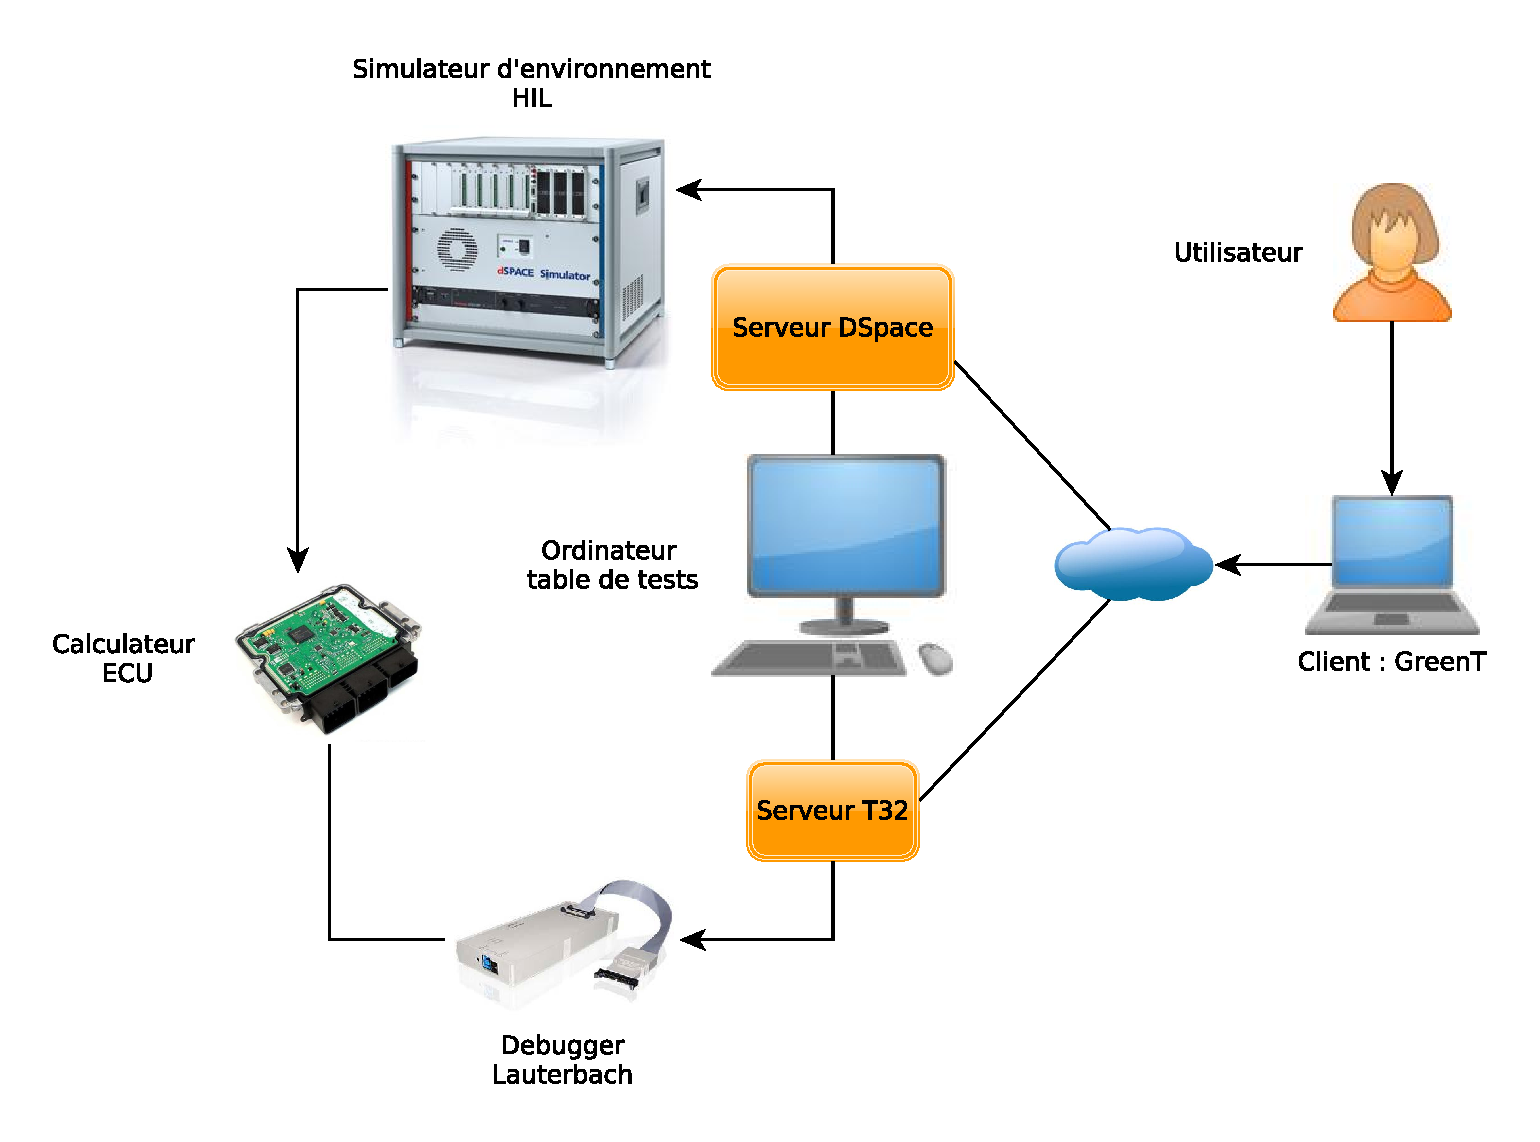
\includegraphics[width=17cm]{contents/images/network.eps}
	\caption{Communications de la plateforme}
	\label{fig:wbgt}
\end{figure}

Au début du développement de la plateforme, il a été décidé que les serveurs devront être le plus simple possible pour plusieurs raisons
: 
\begin{itemize}
	\item Donner accès à un maximum de fonctionnalités en mode << offline >>, c'est-à-dire sans accès à une table de test
	\item Rabattre le maximum de fonctions métier près du client pour centraliser au maximum le fonctionnement et éviter la maintenance superflue
	\item Avoir la possibilité de réutiliser les serveurs pour d'autres projets
	\item Pouvoir ajouter facilement un nouveau \textit{device}, qui ne nécessiterai que l'ajout d'un nouveau serveur relativement simple
\end{itemize}

\subsection{Le serveur Debugger, contrôle de Trace32}\label{T32server}
Le serveur Debugger propose des services basiques permettant de répondre aux besoins :
\begin{itemize}
	\item Flasher le logiciel dans la flash de l'ECU
	\item Démarrer l'ECU
	\item Arrêter l'ECU
	\item Lire une variable ou une calibration
	\item Modifier une variable
	\item Enregistrer des variables
\end{itemize}~

\begin{wrapfigure}{l}{3cm}
	\vspace{-40px}
	
\includegraphics[width=2.5cm]{contents/images/logoJava.png}
\end{wrapfigure}
Afin d'effectuer ces actions, le serveur s'appuie sur une API fournie par l'outil Trace32 permettant de contrôler le debugger. Ainsi tous nos services vont s'appuyer sur cette API. C'est pour cette raison que ce serveur est développé en Java afin de pouvoir utiliser
facilement ces fonctions.

\subsection{Le serveur HiL, contrôle du ControlDesk DSPace}
Le HiL contient une base de données, représentant un modèle simulant l'environnement véhicule. Ce modèle à pour but de se rapprocher au maximum du fonctionnement réel de notre moteur.

Le serveur DSpace va devoir lui aussi répondre aux différentes stimulations, ainsi ces services sont relativement similaire : 
\begin{itemize}
	\item Modifier une valeur du modèle
	\item Lire une valeur du modèle
	\item Enregistrer des valeurs
\end{itemize}~

\begin{wrapfigure}{r}{3cm}
	
\includegraphics[width=2.5cm]{contents/images/python.png}
\end{wrapfigure}
Ce serveur a été développé en réutilisant une partie de ce qui avait été fait pour la TA3, présenté section \ref{ta3} afin de ne pas
<< réinventer la roue >>. 

À l'instar du serveur Debugger, nous utilisons une API fournie par l'outil permettant de contrôler le HIL : ControlDesk. 
C'est ainsi que ce serveur est développé en Python afin de répondre à cette contraintes : l'API du ControlDesk est en Python. Ainsi, l'utilisation de Thrift, permettant de faire dialoguer du Java côté client et du Python côté serveur facilement, nous aura particulièrement aidé.


